\documentclass{beamer}
%\usetheme[numbering=none]{metropolis}           % Use metropolis theme
\usetheme{metropolis}           % Use metropolis theme
\title{Cumulative Prospect Theory Meets Reinforcement Learning:\\ Prediction and Control}
\date{}
\author{Prashanth L.A.\\[1.5ex]
{\footnotesize Joint work with Cheng Jie, Michael Fu, Steve Marcus and Csaba Szepesv\'ari}}
\institute{University of Maryland, College Park}

\usepackage{macros}

\begin{document}
 
\maketitle
%%%%%%%%%%%%%%%%%%%%%%%%%%%%%%%%%%%%%%%%%%%%%%%%

\begin{frame}{Human-based decision making system}

\begin{center}
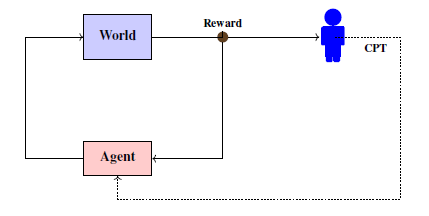
\includegraphics[width=4in]{fig/human_system.png}
\end{center}

\begin{small}
\tikz[baseline]{
            \node[fill=red!20,anchor=base] (t1)
{\makecell{\textit{Cumulative prospect theory (CPT) captures \textbf{human preferences}}}};}
\end{small}

\end{frame}

%%%%%%%%%%%%%%%%%


%

\begin{frame}{CPT-value}
\begin{small}

\textbf{\small\color{bleu1} For a given r.v. $X$, CPT-value $\C(X)$ is}
\begin{align*}
\tikz[baseline]{
            \node[fill=green!20,anchor=base] (t1)
            {$\C(X):= \underbrace{\intinfinity w^+\left(\Prob{u^+(X)>z}\right) dz}_{\textbf{Gains}} - \underbrace{\intinfinity w^-\left(\Prob{u^-(X)>z}\right) dz}_{\textbf{Losses}}$};        }
\end{align*}
\begin{scriptsize}
\alert{\textbf{Utility functions}} $u^+,u^-:\R\rightarrow \R_+$, $u^+(x)=0$ when $x\le 0$, $u^-(x)=0$ when $x\ge 0$

\alert{\textbf{Weight functions}} $w^+,w^-:[0,1] \rightarrow [0,1]$ with $w(0)=0$, $w(1)=1$
\end{scriptsize}

\pause
\vspace{2ex}

\textbf{\small\color{rouge2} Connection to expected value:} 
\begin{align*}
\tikz[baseline]{
            \node[fill=red!20,anchor=base] (t1)
            {\makecell{$\C(X) = \intinfinity \Prob{X>z} dz -  \intinfinity \Prob{-X>z} dz$\\[1ex]
						\hspace{-3em}$= \EE{ (X)^+ } - \EE{ (X)^- }$}};
        }
\end{align*}
{\scriptsize$(a)^+ = \max(a,0)$, $(a)^- = \max(-a,0)$}
\end{small}



\end{frame}


%%%%%%%%%%%%%%%%%%%%%%%%%%%%%%%%%%%%%%%%%%%%%%%%
\begin{frame}{Utility and weight functions}
\begin{columns}
 \begin{column}{0.48\textwidth}
\textbf{\color{bleu1}\small Utility functions}\\[2ex]

   \scalebox{0.5}{\begin{tikzpicture}
   \begin{axis}[width=11cm,height=6.5cm,legend pos=south east,
          %  grid = major,         
            axis lines=middle,
           % grid style={dashed, gray!30},
            xmin=-5,     % start the diagram at this x-coordinate
            xmax=5,    % end   the diagram at this x-coordinate
            ymin=-4,     % start the diagram at this y-coordinate
            ymax=4,   % end   the diagram at this y-coordinate
           % axis background/.style={fill=white},
            ylabel={\large\bf Utility},
            xlabel={\large\bf Gains},
            x label style={at={(axis cs:4.7,-0.8)}},
            y label style={at={(axis cs:-0.8,4.8)}},
            xticklabels=\empty,
            yticklabels=\empty
            ]
           \addplot[name path=cptplus,domain=0:5, green!35!black, very thick,smooth] 
              {pow(abs(x),0.8)}; 
            \addplot[name path=cptminus,domain=-5:0, red!35!black,very thick,smooth] 
              {-2*pow(abs(x),0.7)}; 
               \addplot[domain=-5:5, blue, thick]           {x}; 
               
               \path[name path=diagplus] (axis cs:0,0) -- (axis cs:5,5);
 			  \path[name path=diagminus] (axis cs:-5,-5) -- (axis cs:0,0);
                \path[name path=xaxisplus] (axis cs:0,0) -- (axis cs:5,0);
                 \path[name path=xaxisminus] (axis cs:-5,0) -- (axis cs:0,0);
                 \path[name path=yaxisplus] (axis cs:0,0) -- (axis cs:0,5);
                 \path[name path=yaxisminus] (axis cs:0,-5) -- (axis cs:0,0);
 
 \addplot [orange!40]  fill between[of= diagminus and yaxisminus];
 \addplot [cyan!20]  fill between[of= diagplus and xaxisplus];
 
 \node at (axis cs:  -3.7,-0.45) {\large\bf Losses};
 \node at (axis cs:  4,2.5) {\large $\bm{u^+}$};
 \node at (axis cs:  -1,-3) {\large $\bm{-u^-}$};
 %\node at (axis cs:  2.5,-2.5) {\large\bf Reference point};
%\draw[-{>[scale=2.5,
          %length=5,
          %width=3]},thick] (axis cs:2,-2) -- (axis cs:0,0);
   \end{axis}
   \end{tikzpicture}}

%A reference point on the $x$ axis serves as the point of separating gains and losses.
%For losses, the disutility $-u^-$ is typically convex, for gains, the utility $u^+$ is typically concave; 
%they are always non-decreasing and both of them take on the value of zero at the reference point.
\begin{center}
\begin{scriptsize}
\tikz[baseline]{
            \node[fill=red!20,anchor=base] (t1)
{\makecell{For losses, the disutility $-u^-$ is \textbf{convex},\\
 for gains, the utility $u^+$ is \textbf{concave}}};}
\end{scriptsize}
\end{center}

 \end{column}
 \begin{column}{0.48\textwidth}
\textbf{\color{bleu1}\small Weight function}\\[2ex]

  \scalebox{0.55}{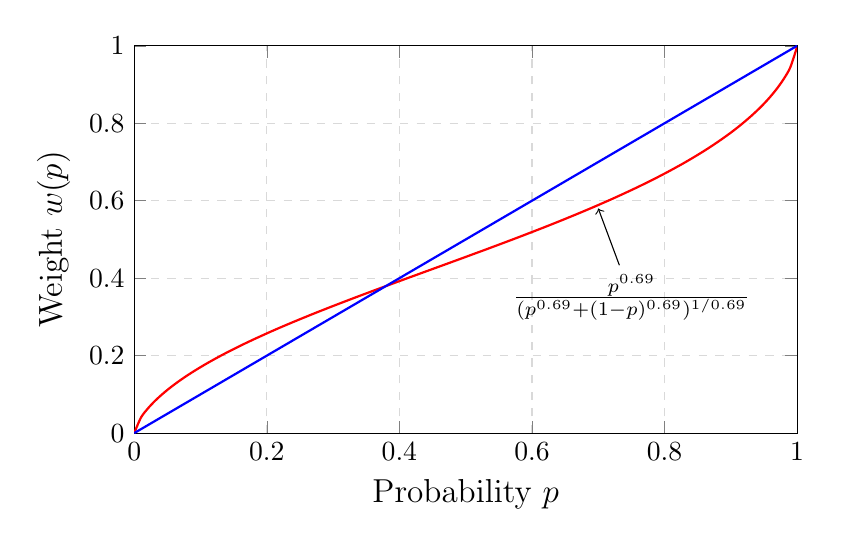
\begin{tikzpicture}
  \begin{axis}[width=10cm,height=6.5cm,legend pos=south east,
           grid = major,
           grid style={dashed, gray!30},
           xmin=0,     % start the diagram at this x-coordinate
           xmax=1,    % end   the diagram at this x-coordinate
           ymin=0,     % start the diagram at this y-coordinate
           ymax=1,   % end   the diagram at this y-coordinate
           axis background/.style={fill=white},
           ylabel={\large Weight $\bm{w(p)}$},
           xlabel={\large Probability $\bm{p}$}
           ]
          \addplot[domain=0:1, red, thick,smooth, samples=100] 
             {pow(x,0.69)/pow((pow(x,0.69) + pow(1-x,0.69)),1.44)}; 
             \node at (axis cs:  0.75,0.35) (a1) {$\bm{\frac{p^{0.69}}{(p^{0.69}+ (1-p)^{0.69})^{1/0.69}}}$};           
             \draw[->] (a1) -- (axis cs:  0.7,0.58);
                 \addplot[domain=0:1, blue, thick]           {x};                      
  \end{axis}
  \end{tikzpicture}}
\begin{center}
\begin{scriptsize}
\tikz[baseline]{
            \node[fill=red!20,anchor=base] (t1)
{\makecell{\textbf{Overweight} low probabilities,\\
 \textbf{underweight} high probabilities}};}
\end{scriptsize}
\end{center}

\end{column}
\end{columns}



\end{frame}

\begin{frame}{Prospect Theory}

\begin{columns}
 \begin{column}{0.35\textwidth}

\includegraphics[height=1.5in]{fig/tversky.jpg}  

\textbf{~Amos Tversky}
 \end{column}

 \begin{column}{0.35\textwidth}

\includegraphics[height=1.5in]{fig/kahneman.jpeg}  

\textbf{~Daniel Kahneman}
 \end{column}
\end{columns}

\vspace{7ex}

\begin{scriptsize}
  Kahneman \& Tversky (1979) ``\textit{Prospect Theory: An analysis of decision under risk}'' is the second most cited paper in economics during the period, 1975-2000 
\end{scriptsize}

\end{frame}

%%%%%%%%%%%%%%%%%% Contrib %%%%%%%%%%%%%%%%%%%%%%%%%%%%
\begin{frame}{Our Contributions}
\begin{small}
\begin{scriptsize}
\begin{align*}
\tikz[baseline]{
            \node[fill=green!20,anchor=base] (t1)
            {${\cal C} (X^\theta):= \underbrace{\intinfinity w^+(P(u^+(X^\theta))>x) dx}_{\textbf{Gains}} - \underbrace{\intinfinity w^-(P(u^-(X^\theta))>x) dx}_{\textbf{Losses}}$};
        }
\end{align*}
  \begin{center}
\tikz[baseline]{
            \node[fill=magenta!20,anchor=base] (t1)
            {$\textrm{Find ~}\theta^* = \argmax_{\theta \in \Theta} \C(X^\theta)$};
        }\end{center}
\end{scriptsize}

\begin{itemize}
	\item CPT-value estimation using \alert{\footnotesize\bf\em empirical distribution functions}
	\item SPSA-based \begin{footnotesize}\alert{\bf\em policy gradient}\end{footnotesize}  algorithm
	\item sample complexity bounds for estimation + \begin{footnotesize}\alert{\bf\em asymptotic convergence}\end{footnotesize} of policy gradient
	\item \begin{footnotesize}\alert{\bf\em traffic signal control}\end{footnotesize} application
\end{itemize}
\end{small}

\end{frame}
%%%%%%%%%%%%%%%%%%%%%%%%%%%%%%%%%%%%%%%%%%%%%%%%

%%%%%%%%%%%%%%%%% Estimation %%%%%%%%%%%%%%%%%%%%%%%%%
\begin{frame}{CPT-value estimation}
\begin{small}

{\color{red} Problem:} Given samples $X_1, \ldots, X_n$ of $X$, estimate
%
\begin{align*}
\tikz[baseline]{
            \node[fill=blue!20,anchor=base] (t1)
            {$\C(X):= \intinfinity w^+\left(\Prob{u^+(X)>z}\right) dz - \intinfinity w^-\left(\Prob{u^-(X)>z}\right) dz$};
        }
\end{align*}

\vspace{0.25in}
%\pause

\tikz[baseline]{
            \node[fill=red!20,anchor=base] (t1)
            {\textbf{Nice to have}: Sample complexity $O\left(1/\epsilon^2\right)$ for accuracy $\epsilon$};
        }
				
\end{small}				
\end{frame}



%%%%%%%%%%%%%%%%% Estimation %%%%%%%%%%%%%%%%%%%%%%%%%
\begin{frame}{}

\vspace{1ex}

\begin{small}
\alert{Empirical distribution function (EDF):} Given samples $X_1, \ldots, X_n$ of $X$, 
%
\begin{align*}
\tikz[baseline]{
            \node[fill=blue!20,anchor=base] (t1)
            {${\hat F_n}^+(x)=\frac{1}{n} \sum_{i=1}^n 1_{(u^+(X_i) \leq x)}, \quad\text{and}\quad {\hat F_n}^-(x)=\frac{1}{n} \sum_{i=1}^n 1_{(u^-(X_i) \leq x)}$};
        }
\end{align*}

\vspace{1ex}
%\pause

Using EDFs, the CPT-value $\C(X)$ is estimated by
\begin{align*}
\tikz[baseline]{
            \node[fill=red!20,anchor=base] (t1)
            {
$\overline \C_n = \underbrace{\intinfinity w^+(1-{\hat F_n}^+(x))  dx}_{\textbf{Part (I)}} - \underbrace{\intinfinity w^-(1-{\hat F_n}^-(x))  dx}_{\textbf{Part (II)}}$
};
        }
        \end{align*}

\pause

\alert{Computing Part (I):} Let $X_{[1]}, X_{[2]}, \ldots ,X_{[n]}$ denote the order-statistics 				
        \begin{align*}
\tikz[baseline]{
            \node[fill=green!20,anchor=base] (t1)
            {
$\textbf{Part (I)} = \sum_{i=1}^{n} u^+(X_{[i]}) \left(w^+\!\left(\frac{n+1-i}{n}\right)\!-\! w^+\!\left(\frac{n-i}{n}\right) \right),$
};
        }
        \end{align*}
				
\end{small}
\end{frame}

%%%%%%%%%%%%%%%%% Estimation %%%%%%%%%%%%%%%%%%%%%%%%%

\begin{frame}{	}

\vspace{3ex}

\begin{small}

%\begin{scriptsize}
{\textbf{(A1).}  Weights $w^+, w^-$ are \holder continuous, i.e., $| w^+(x) - w^+(y) | \leq H | x-y |^{\alpha}$, $\forall x,y \in [0,1]$}\\[2ex]
{\textbf{(A2).}  Utilities $u^+(X)$ and $u^-(X)$ are bounded above by $M<\infty$}\\[4ex]

{\color{blue}\textbf{Sample Complexity:}}\\[1ex]
Under (A1) and (A2), for any $\epsilon, \delta >0$, we have
\begin{align*}
\tikz[baseline]{
            \node[fill=pink!20,anchor=base] (t1)
            {
$\Prob{\left |\overline \C_n- \C(X) \right| \leq  \epsilon } >1- \delta\text{     ,} \forall n \geq \ln\left(\frac{1}{\delta}\right)\cdot 
\frac{4H^2 M^2}{\epsilon^{2/\alpha}}$};}
\end{align*}
%\end{scriptsize}

\vspace{3ex}
\pause

\tikzstyle{block} = [draw, fill=white, rectangle,
   minimum height=5em, minimum width=6em]
\tikzstyle{sum} = [draw, fill=white, circle, node distance=1cm]
\tikzstyle{input} = [coordinate]
\tikzstyle{output} = [coordinate]
\tikzstyle{pinstyle} = [pin edge={to-,thin,black}]

\begin{columns}
\begin{column}{0.5\textwidth}
\scalebox{0.6}{\begin{tikzpicture}[auto, node distance=2cm,>=latex']
% We start by placing the blocks
\node (theta) {$\boldsymbol{x}$};
\node [block, fill=blue!20,right=0.6cm of theta,align=center] (sample) {\makecell{\textbf{Measurement}\\\textbf{ Oracle}}}; 
\node [right=0.6cm of sample] (end) {$\boldsymbol{\mathbf{f(x) + \xi}}$};
\node [ above right= 0.6cm of end] (bias) {\textbf{Zero mean}};
\draw [->] (theta) --  (sample);
\draw [->] (sample) -- (end);
\path [darkgreen,->] (bias) edge [bend left] (end);
\end{tikzpicture}}

\hspace{2em}{\scriptsize Simulation optimization}
\end{column}
\begin{column}{0.5\textwidth}
\scalebox{0.6}{\begin{tikzpicture}[auto, node distance=2cm,>=latex']
% We start by placing the blocks
\node (theta) {$\boldsymbol{X, \epsilon}$};
\node [block, fill=blue!20,right=0.6cm of theta,align=center] (sample) {\makecell{\textbf{CPT}\\\textbf{ Estimator}}}; 
\node [right=0.6cm of sample] (end) {$\boldsymbol{\mathbf{\C(X) + \epsilon}}$};
\node [ above right= 0.6cm of end] (bias) {\textbf{Controlled bias}};
\draw [->] (theta) --  (sample);
\draw [->] (sample) -- (end);
\path [red,->] (bias) edge [bend left] (end);
\end{tikzpicture}}

\hspace{1em}{\scriptsize CPT-value optimization}
\end{column}
\end{columns}

\end{small}
\end{frame}


%%%%%%%%%%%%%%%%%%%%%%%%%%%%%%%%%%%%%%%%%%%%%%%%
%%%%%%%%%%%%%%%%%%%%%%%%%%%%%%%%%%%%%%%%%%%%%%%%

\begin{frame}{CPT-value optimization}
  \begin{small}

	\onslide<1->{
  \centering
\tikz[baseline]{
            \node[fill=magenta!20,anchor=base] (t1)
            {$\textrm{Find ~}\theta^* = \argmax_{\theta \in \Theta} \C(X^\theta)$};
        }
}
\ \\[3ex]
\textbf{\color{bleu2} RL application:} $\theta = $ policy parameter,  $X^\theta = $ return
\\[6ex]
	
\begin{columns}
 \begin{column}{0.4\textwidth}
      %\begin{figure}
      \tikzset{
	  %Define standard arrow tip
	  >=stealth',
	  %Define style for boxes
	  punkt/.style={
		rectangle,
		rounded corners,
		draw=black, very thick,
		text width=7.5em,
		minimum height=3.5em,
		text centered},
	  % Define arrow style
	  pil/.style={
		->,
		thick,
		shorten <=2pt,
		shorten >=2pt,}
      }
      %\textbf{Policy iteration principle central to LSPI}
      \centering
      \scalebox{0.65}{\begin{tikzpicture}[node distance=1cm, auto,]
      %nodes
      \node (dummy) {};
      \node[punkt,fill=blue!20,above=1cm of dummy] (peval) {\bf Prediction};
      \node[punkt, fill=red!20,inner sep=5pt,below=1cm of dummy]
      (pimp) {\bf Control};
      % We make a dummy figure to make everything look nice.
      \node[right=2cm of dummy] (t) {\bf CPT-value $\bm{\C^\theta}$}
	edge[pil,<-,bend right=45] (peval.east) % edges are used to connect two nodes
	edge[pil, bend left=45] (pimp.east); % .east since we want
						  % consistent style
      \node[left=2cm of dummy] (g) {\bf Parameter $\bm{\theta}$}
	edge[pil, bend left=45] (peval.west)
	edge[pil,<-, bend right=45] (pimp.west);
      \end{tikzpicture}}
      %\caption{Overall flow of CPT-value optimizing algorithms}

      %\end{figure}
  
 \end{column}
 \begin{column}{0.05\textwidth}
 \end{column}
 \begin{column}{0.45\textwidth}
\onslide<1>{
{\bf\color{darkgreen} Two-Stage Solution:}
\begin{description}
 \item[{\color{darkgreen} inner stage}] Obtain samples of $X^{\theta}$ and estimate $\C(X^{\theta})$;
% \vspace{-1.5ex}
 \item[{\color{darkgreen} outer stage}] Update $\theta$ using gradient ascent 
% \vspace{-1.5ex}
\end{description}
\alert{~~$\nabla_{i} \C(X^\theta)$ is not given}
}
 \end{column}
\end{columns}
\end{small}
\end{frame}


%%%%%%%%%%%%%%%%%%
\begin{frame}{}
\begin{small}
\begin{equation*}
\textbf{\color{blue!80} Update rule:} \quad \theta^{i}_{n+1} = 
        \tikz[baseline]{
            \node[fill=blue!20,ellipse,anchor=base] (t0)
            {$\Gamma_{i}$};
        } 
\bigg(\theta^{i}_n  +
        \tikz[baseline]{
            \node[fill=blue!20,ellipse,anchor=base] (t1)
            {$\gamma_n$};
        } 
        \tikz[baseline]{
            \node[fill=red!20, anchor=base] (t2)
            {$\widehat \nabla_{i} \C(X^{\theta_n})$};
        }\bigg),   \quad i=1,\ldots, d.
\end{equation*}

\vspace{0.5cm}

\begin{tabular}[b]{ccc}
\begin{minipage}{0.3\textwidth}
\centering
\tikz[na]\node [coordinate] (n0) {};\textbf{\color{bleu1} Projection operator}           
\end{minipage} 
&
\begin{minipage}{0.3\textwidth}
\centering
\textbf{\color{bleu2} Step-sizes} \tikz[na]\node [coordinate] (n1) {};          
\end{minipage} 
&
\begin{minipage}{0.3\textwidth}
\centering
\tikz[na]\node [coordinate] (n2) {};  \textbf{\color{vert4}     Gradient estimate} 
\end{minipage}
%\\[0.5cm]
% \multicolumn{2}{c}{
%\tikz[baseline]{\node[fill=green!30] {\bf \color{darkgreen!70!black} Complexity: $O(d)$ per iteration };}} 
\end{tabular}

\begin{tikzpicture}[overlay]
        \path[->] (n0) edge [out=145,in=-90] (t0);
        \path[->] (n1) edge [bend right] (t1);
        \path[->] (n2) edge [bend left] (t2);
\end{tikzpicture}

%$\alt<2>{\frac{(x^2+1)\sqrt{x+3}}{x-1}}{y}$

\alert{\textbf{Challenge}:} {estimating $\nabla_{i} \C(X^\theta)$
given only biased estimates of $\C(X^\theta)$}

\vspace{3.5ex}

{\bf\color{darkgreen} Solution: use SPSA [Spall'92]}
\begin{align*}
% \label{eq:SPSA-grad}
\widehat \nabla_{i} \C(X^\theta) = \dfrac{\overline \C_n^{\theta_n+\delta_n \Delta_n} - \overline \C_n^{\theta_n-\delta_n \Delta_n}}{2 \delta_n \Delta_n^{i}}
\end{align*}
{\scriptsize$\Delta_n$ is a vector of independent Rademacher r.v.s and $\delta_n>0$ vanishes asymptotically.}

\end{small}
\end{frame}
%%%%%%%%%

\begin{frame}{Application: Traffic signal control}
\begin{columns}
	\begin{column}{0.4\textwidth}
	        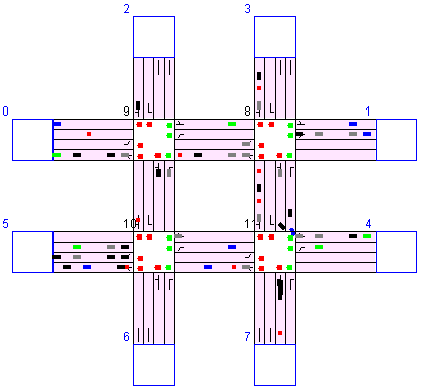
\includegraphics[width=2in, height=1.2in]{fig/2x2grid.png}
	\end{column}
	\begin{column}{0.53\textwidth}
	\begin{small}
	\begin{itemize}
		\item For any path $i=1,\ldots,\M$, let $X_i$ be the differential delay 
		\begin{itemize}
			\item {\scriptsize calculated with a pre-timed traffic light controller as reference}
		\end{itemize} 
		\item CPT captures the road users' evaluation of the delay $X_i$
		\item Goal: Maximize \tikz[baseline]{
            \node[fill=red!20, anchor=base] (t2)
            {$\text{CPT}(X_1,\ldots,X_{\M}) = \sum_{i=1}^{\M} \mu^i \C(X_i)$};
        }
				
				$\mu^i$: proportion of traffic on path $i$
	\end{itemize}
	\end{small}
	\end{column}
\end{columns}

\end{frame}
%%%%%%%%%%%%%%%%%%%%%%%%%%%%%%%%%%%%%%%%%%%%%%%%
\begin{frame}{}
 \begin{figure}

\vspace{-2.5ex}

    \centering
     \begin{tabular}{ccc}
\subfigure[AVG-SPSA]{
\label{fig:avg}
%\hspace{2em} 
\tabl{c}{\scalebox{0.45}{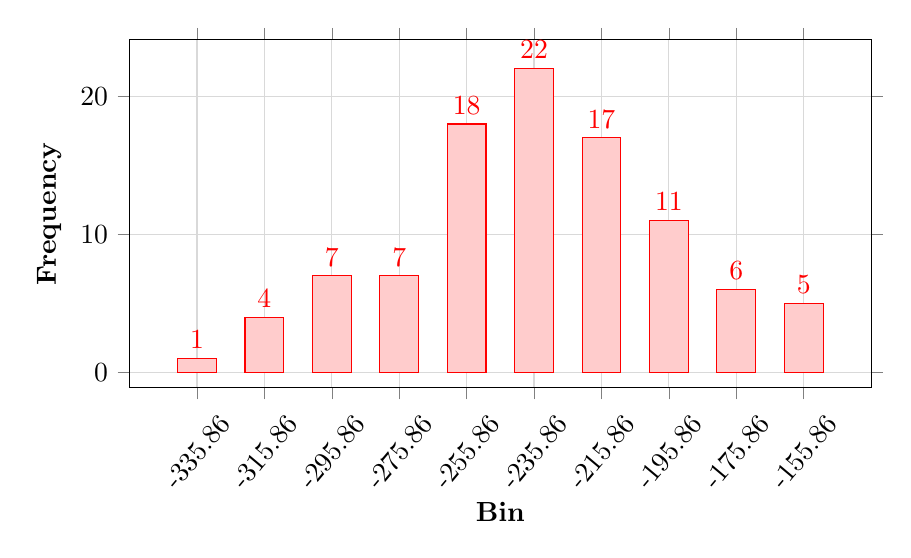
\begin{tikzpicture}
\begin{axis}[
ybar={2pt},
%  legend style={at={(0.5,-0.2)},anchor=north,legend columns=-1},
legend pos=outer north east,
legend image code/.code={\path[fill=white,white] (-2mm,-2mm) rectangle
(-3mm,2mm); \path[fill=white,white] (-2mm,-2mm) rectangle (2mm,-3mm); \draw
(-2mm,-2mm) rectangle (2mm,2mm);},
ylabel={\bf Frequency},
xlabel={\textbf{Bin}},
x label style={at={(axis description cs:0.5,-0.3)},anchor=north},
symbolic x coords={0, -335.86, -315.86, -295.86, -275.86, -255.86, -235.86, -215.86, -195.86, -175.86, -155.86, 11},
xmin={0},
xmax={11},
xtick=data,
ytick align=outside,
%xticklabels={{\bf7x9-Grid\\[0.5ex]($d=504$),\bf 14x9-Grid\\[0.5ex]($d=1008$),\bf 14x18-Grid\\[0.5ex]($d=2016$),\bf 28x18-Grid\\[0.5ex]($d=4032$)}},
xticklabel style={rotate=50, align=center},
bar width=14pt,
nodes near coords,
grid,
grid style={gray!30},
width=11cm,
height=6cm,
]
\addplot[red, fill=red!20]   coordinates {  (-335.86,1) (-315.86,4) (-295.86,7) (-275.86,7) (-255.86,18) (-235.86,22) (-215.86,17) (-195.86,11) (-175.86,6) (-155.86,5)}; %LSPI
\end{axis}
\end{tikzpicture}}\\[1ex]}
}
&
%%%%%%%%%%%%%%
\subfigure[EUT-SPSA]{
\label{fig:eut}
%\hspace{2em} 
\tabl{c}{\scalebox{0.45}{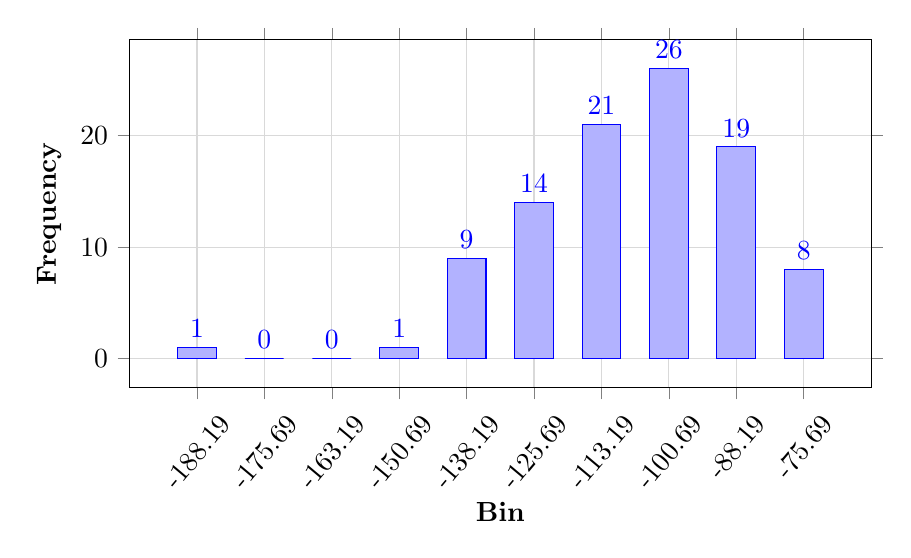
\begin{tikzpicture}
\begin{axis}[
ybar={2pt},
%  legend style={at={(0.5,-0.2)},anchor=north,legend columns=-1},
legend pos=outer north east,
legend image code/.code={\path[fill=white,white] (-2mm,-2mm) rectangle
(-3mm,2mm); \path[fill=white,white] (-2mm,-2mm) rectangle (2mm,-3mm); \draw
(-2mm,-2mm) rectangle (2mm,2mm);},
ylabel={\bf Frequency},
xlabel={\textbf{Bin}},
x label style={at={(axis description cs:0.5,-0.3)},anchor=north},
symbolic x coords={0,-188.19,-175.69,-163.19,-150.69,-138.19,-125.69,-113.19,-100.69,-88.19,-75.69,11},
xmin={0},
xmax={11},
xtick=data,
ytick align=outside,
%xticklabels={{\bf7x9-Grid\\[0.5ex]($d=504$),\bf 14x9-Grid\\[0.5ex]($d=1008$),\bf 14x18-Grid\\[0.5ex]($d=2016$),\bf 28x18-Grid\\[0.5ex]($d=4032$)}},
xticklabel style={rotate=50, align=center},
bar width=14pt,
nodes near coords,
grid,
grid style={gray!30},
width=11cm,
height=6cm,
]
\addplot   coordinates {  (-188.19,1) (-175.69,0) (-163.19,0) (-150.69,1) (-138.19,9) (-125.69,14) (-113.19,21) (-100.69,26) (-88.19,19) (-75.69,8) }; %LSPI
\end{axis}
\end{tikzpicture}}\\[1ex]}
}
\end{tabular}
\begin{tabular}{c}
%%%%%%%%%%%%%%%%%%%%%%%%%
\subfigure[CPT-SPSA]{
\label{fig:cpt}
%\hspace{2em} 
\tabl{c}{\scalebox{0.45}{\begin{tikzpicture}
\begin{axis}[
ybar={2pt},
%  legend style={at={(0.5,-0.2)},anchor=north,legend columns=-1},
legend pos=outer north east,
legend image code/.code={\path[fill=white,white] (-2mm,-2mm) rectangle
(-3mm,2mm); \path[fill=white,white] (-2mm,-2mm) rectangle (2mm,-3mm); \draw
(-2mm,-2mm) rectangle (2mm,2mm);},
ylabel={\bf Frequency},
xlabel={\textbf{Bin}},
x label style={at={(axis description cs:0.5,-0.25)},anchor=north},
symbolic x coords={0, -43.36,-33.36,-23.36,-13.36,-3.36,6.64,16.64,26.64,36.64,46.64, 11},
xmin={0},
xmax={11},
xtick=data,
ytick align=outside,
%xticklabels={{\bf7x9-Grid\\[0.5ex]($d=504$),\bf 14x9-Grid\\[0.5ex]($d=1008$),\bf 14x18-Grid\\[0.5ex]($d=2016$),\bf 28x18-Grid\\[0.5ex]($d=4032$)}},
xticklabel style={rotate=50, align=center},
bar width=14pt,
nodes near coords,
grid,
grid style={gray!30},
width=11cm,
height=6cm,
]
\addplot[darkgreen, fill=darkgreen!20]   coordinates {  (-43.36,1) (-33.36,0) (-23.36,0) (-13.36,1) (-3.36,0) (6.64,1) (16.64,8) (26.64,52) (36.64,24) (46.64,12) }; %LSPI
\end{axis}
\end{tikzpicture}}\\[1ex]}
}
\end{tabular}
\caption{Histogram of CPT-value of the differential delay: AVG uses plain sample means (no utility/weights), EUT uses utilities but no weights and CPT uses both utilites and weights. }
\label{fig:histogram-perf}
\end{figure}
	
\end{frame}

\begin{frame}
\begin{center}
\LARGE{Thanks! Questions?}
\end{center}
\end{frame}


\end{document}
